% !TeX encoding = UTF-8
% !TeX program = pdflatex
% !BIB program = bibtex




%\usepackage[english]{babel}
%\usepackage{dsthesis}

\usepackage{verbatim}

\usepackage{algorithm}
\usepackage[noend]{algpseudocode}
\usepackage{algorithmicx}


\usepackage{framed}
\usepackage{todonotes}
\usepackage{graphicx}
\usepackage{multirow}
\usepackage{tocloft}
\usepackage{longtable}
\usepackage{booktabs}
\usepackage{microtype}

%\usepackage{amssymb,amsmath,amsthm,amsfonts}
\usepackage{amsmath,amsfonts}
\newtheorem{definition}{Definition}
\newenvironment{proof}{\paragraph{Proof:}}{\hfill$\square$}
\newtheorem{theorem}{Theorem}

% DRAFT TOOLS
%\geometry{showframe}
\usepackage{todonotes}


\begin{document}
%%% Mehrere Autoren werden durch \and voneinander getrennt.
%%% Die Fußnote enthält die Adresse sowie eine E-Mail-Adresse.
%%% Das optionale Argument (sofern angegeben) wird für die Kopfzeile verwendet.
\title[Extending K-Means Clustering with Ptolemy’s Inequality]{Extending K-Means Clustering with Ptolemy’s Inequality
\thanks{This work is partly funded by DFG grant No. 454630593: EPIX – Efficient Ptolemaic Indexing.} 
}
%% \subtitle{Untertitel / Subtitle} % if needed
\author[1]{Max Pernklau}{max.pernklau@fernuni-hagen.de}{0009-0007-5520-4093}
\author[1]{Nikita Averitchev}{naveritchev@gmail.com}{}
\author[1]{Christian Beecks}{christian.beecks@fernuni-hagen.de}{0009-0000-9028-629X}
% \author[1]{Firstname4 Lastname4}{firstname4.lastname4@affiliation1.org}{0000-0000-0000-0000}%
\affil[1]{FernUniversität in Hagen\\Chair of Data Science\\ 58084 Hagen\\Germany}



\maketitle
\begin{abstract}
	Clustering is a fundamental data analytics operation in the field of unsupervised learning. Given a database of unknown structure, clustering aims to discover the inherent structure of the data objects according to similarity, such that similar data objects are grouped together, while dissimilar ones are separated in different groups or clusters.
	In this study, we focus on partitioning methods, specifically the \emph{k-means clustering} approach, which minimizes the intra-cluster variance.
	As the standard algorithmic approach to k-means clustering, the Lloyd algorithm, is neither efficient nor scalable, various adaptations and modifications have been developed, resulting in the family of fast k-means clustering algorithms.\\
    In this short paper, we extend the clustering algorithm proposed by Elkan with Ptolemy's inequality to prune superfluous distance calculations. It is not our intention to compete with the state-of-the-art algorithmic solutions for the k-means clustering problem; rather, we seek to investigate the potential of Ptolemy’s inequality to further enhancements in the standard algorithm’s performance, particularly in terms of reducing computations associated with distance evaluations.

	% neither tri → pto nor pto → tri is true
	% which generalizes the triangle inequality,

	%where the Lloyd algorithm is a prominent and de facto standard implementation.

	%The resulting groups, which are denoted as clusters, then represent the clustering structure of the database. A

\end{abstract}
\begin{keywords}
	k-means clustering \and Lloyd algorithm \and Ptolemy's inequality %Keyword1 \and Keyword2
\end{keywords}
%%% Beginn des Artikeltexts

%\todo{Americanize spelling (thesis uses chiefly British terms)}

\section{Introduction}

%intro
Clustering is a fundamental data-analytics operation in the domain of data science.
The basic task is to divide a set of data objects into different groups or clusters, such that objects within the same cluster have sufficient similarities;
meanwhile objects in different clusters should have significant differences.
The collection of clusters reflects the inherent structure of the underlying data-generating process and is denoted as a clustering.

The need for clustering arises in various scientific or economic application domains \cite{ezugwu2022comprehensive,oyewole2023data, gan2020data}, ranging from archaeology \cite{troiano2024comparative} and finance \cite{cai2016clustering} to industry \cite{lee2021technological} and zoology \cite{shen2021multivariate}, to name just a few. Especially in the field of unsupervised learning, clustering is utilized to extract structures from unlabeled data \cite{chander2023data}.

Alongside the diverse applications of clustering, unique domain-specific requirements and challenges arise, which are addressed by leveraging different families of clustering approaches \cite{xu2015comprehensive,han2012data}. These approaches, ranging from partitioning and hierarchical methods to density-based, grid-based and graph-based methods, are designed to accommodate varying data characteristics and domain-related requirements to facilitate efficient cluster analyses across diverse applications.

%different algorithms/problems
%kmeans/lloyd
%fast algorithms
%inefficient: distance calculations
%our proposal: ptolemaic
%our purpose

In this short paper, we focus on partitioning methods due to their simplicity in terms of interpretability and implementability \cite{DBLP:conf/iiwas/BeecksBHLSD22}. In this field, the \emph{k-means algorithm} \cite{bock2007clustering,hans2008origins,DBLP:journals/prl/Jain10,steinley2006k} has become one of the most influential clustering techniques \cite{DBLP:journals/kais/WuKQGYMMNLYZSHS08,olukanmi2019rethinking}. Although the term \emph{k-means algorithm} is explicitly credited to MacQueen \cite{macqueen1967}, its origins trace back to Steinhaus \cite{steinhaus1956division} in 1956, with its first application to data clustering by Forgy \cite{forgy1965cluster} in 1965. The widely recognized version in use today is the \emph{Lloyd algorithm} \cite{DBLP:journals/tit/Lloyd82}, introduced in 1982.

With the proliferation of complex data sources and the growing demand for more efficient clustering techniques, numerous \emph{fast k-means algorithms} have been introduced \cite{DBLP:conf/icml/Elkan03,DBLP:conf/sdm/Hamerly10,drake2012accelerated,hamerly2015accelerating,DBLP:conf/icml/NewlingF16,DBLP:conf/icml/DingZSMM15,DBLP:conf/sisap/SchubertLF21,DBLP:conf/sisap/LangS23}. These methods are designed to achieve good clustering results with significantly reduced computational cost. Moreover, most of them do not require any form of precomputation, making them directly applicable across a wide range of scenarios. The major objective of fast k-means algorithms is to reduce the number of distance evaluations required when assigning data objects to cluster centers and to safely prune cluster centers from the assignment process. For this purpose, distances are approximated via lower and upper bounds.

The Elkan algorithm \cite{DBLP:conf/icml/Elkan03} is a prominent representative of these algorithms and particularly suited for high-dimensional scenarios.
It maintains one upper bound and multiple lower bounds for each data object in order to apply different pruning criteria for each combination of data object and cluster center.
While the lower and upper bounds of Elkan's algorithm are directly derived from the triangle inequality, we propose to utilitze Ptolemy's inequality instead in order to increase the pruning performance.
With this extension, we do not aim to compete with the state of the art in k-means clustering;
rather, we intend to investigate the potential of Ptolemy’s inequality to further enhancements in the standard algorithm’s performance, specifically in terms of reducing computations associated with distance evaluations. We believe that our research findings offer a promising direction for future research and are beneficial for data scientists researchers and practitioners alike.

This short paper is structured as follows:
Section~\ref{Preliminaries} outlines the k-means problem and Elkan's approach of accelerating the algorithmic computation.
In Section~\ref{sec:contrib}, we show how Ptolemy's inequality can be applied to the aforementioned algorithm. %as our main contribution.
The results of our preliminary performance evaluation are detailed in Section~\ref{sec: results}, while Section~\ref{sec: conclusions} concludes this paper with a short outlook on future work.

%contribution

%structure


%\newpage


%\section{Related Work}
%\todo{remove this section if we run out of time}

\newcommand{\kmeans}{$k$-means problem\xspace}

\section{Preliminaries}\label{Preliminaries}

In this section, we first define the k-means clustering problem and the Lloyd algorithm as a solution to this problem in Section \ref{subsec: kmeans}.
We then continue with introducing means of acceleration via lower and upper bounding in Section \ref{sub:acc}.


\subsection{The \kmeans} \label{subsec: kmeans}

In order to discuss the \kmeans, it is sensible to define the concept of a \emph{clustering algorithm} formally.
\begin{definition}[clustering algorithm]
	Given a target number of clusters $k$,
	let $F$ be a function that assigns each element from an input data set $D\subset \mathbb{R}^n$ to a
	cluster index $i \in \{1, 2, \ldots, k\}$
	$$ F:D \to \{1, 2, \ldots, k\} \;.$$
\end{definition}
Notably, we restrict our analysis to clustering problems that use the $n$-dimensional Euclidean space as the domain of the input data set.
Likewise, we assume that the similarity of the data points to be clustered is completely defined by the Euclidean distance $d(x,y)= || x-y ||_2 $.
The rationale behind this assumption will be made clear shortly in \autoref{sub:acc}.

The heart of the \kmeans is the assignment of clusters so that the variance in similarity between all points in the same cluster should be reasonably small.
More formally:
\begin{definition}[\kmeans]
	Let $F$ be a clustering algorithm
	%$x \in D$ be an element from the input data set of a clustering algorithm $F$
	and let $C_i$ be the set of all elements assigned to cluster $i$:
	$$ C_i = \{x \in D \mid F(x) = i\} \,.$$
	Furthermore, let $\epsilon$ be the weighted sum of inter-cluster variances
	$$ \epsilon = \sum_{i=1}^k |C_i| \operatorname{Var}[C_i] = \sum_{i=1}^k \sum_{x_j \in C_i}  d^2(x_j, c_i)\,, $$
	where $c_i = \operatorname{E}[C_i]$ is center of cluster $C_i$.

	Then, the map $F$ is called a solution to the \kmeans
	if $\epsilon$ cannot be made smaller by changing the assignment of any one element to a different cluster.
\end{definition}
Note that with this definition, the common $k$-means algorithms provides solution to the \kmeans,
as we do not require that $F$ finds the smallest possible $\epsilon$,
just a local minimum of $\epsilon$.
This is consistent with the colloquial notion that solutions to the \kmeans ``can be found'',
even when an optimal solution (an NP-hard problem) is not practically obtainable \cite{}.

The most prevalent algorithm employed to identify valid solutions to the \kmeans is the Lloyd algorithm.
For convenience, it is reproduced in \autoref{alg:lloyd};
given its widespread use, we will only cover its most significant characteristics as they relate to our analysis.

\begin{algorithm}[t]
	\caption{k-Means Algorithm}
	\label{alg:lloyd}

	\textbf{Input:} \( k \): Number of clusters, \( D \): Dataset containing \( n \) objects

	\textbf{Output:} Assignment of each $x_i \in D$ to a clusters

	\begin{algorithmic}[1]
		\State Initialize \( k \) cluster centers \( \{c_1, c_2, \dots, c_k\} \) arbitrarily from \( D \)
		\Repeat
		\label{algstep:assign}
		\State \textcolor{gray}{// Assign \( x_i \) to the closest cluster}
		\For{each object \( x_i \) in \( D \)}
		\State \( C_j \leftarrow C_j \cup \{x_i\} \) where \( j = \underset{j}{\arg\min} \; d^2(x_i, c_j) \)
		\EndFor
		\State \textcolor{gray}{// Update cluster center \( c_j \)}
		\For{each cluster \( C_j \)}
		\State \( c_j \leftarrow \frac{1}{|C_j|} \sum_{x_i \in C_j} x_i \)
		\EndFor
		\Until{no change in cluster assignments}
	\end{algorithmic}
\end{algorithm}

For each iteration of Lloyds algorithm, the assignment step (\autoref{algstep:assign}) needs to identify the closest cluster center for each element from the input dataset $D$.
To do so, Lloyd's algorithm calculates the distances between each cluster and each element from $D$, requiring $k\cdot|D|$ total distance evaluations per iteration.
These frequent distance evaluations can make up a significant share of the algorithms computational costs, especially for high-dimensional datasets.


\subsection{Accelerating $k$-means}
\label{sub:acc}

\begin{algorithm}
	\caption{Elkan's Algorithm}
	\label{alg:elkan}
	\begin{algorithmic}
		\State \textbf{Initialization:} Initialize all cluster centers. For each point $x_i$ and each center $c_j$, set the lower bound $l(x_i,c_j)$ and the upper bound $u(x_i)$. Assign each $x_i$ to the nearest cluster $C_j$ such that $c(x_i) = \argmin_j d(x_i, c_j)$, utilizing Lemma 1 to minimize distance calculations. Set $r(x_i) = \text{true}$ for all points.
		\todo{include Lemma 1}

		\Repeat
		\State \textbf{Step 1:} Compute distances $d(c_i, c_j)$ between all centers, and calculate $s(c_i) = \frac{1}{2} \min_{c_j \neq c_i} d(c_i, c_j)$ for each center $c_i$.

		\State \textbf{Step 2:} Retain points $x_i$ in their current clusters if $u(x_i) \leq s(c(x_i))$.

		\State \textbf{Step 3:} For remaining points, consider $x_i$ for reassignment if:
		\begin{itemize}[leftmargin=5em,itemindent=\algorithmicindent,itemsep=0pt,parsep=0pt]
			\item $c_j \neq c(x_i)$,
			\item $u(x_i) > l(x_i, c_j)$, and
			\item $u(x_i) > 0.5 \cdot d(c(x_i), c_j)$.
		\end{itemize}

		\State \textbf{Step 3a:} If $r(x_i)$ is true, compute $d(x_i, c(x_i))$. Set $r(x_i) = \text{false}$. Otherwise, $u(x_i) = d(x_i, c(x_i))$.

		\State \textbf{Step 3b:} If $d(x_i, c(x_i)) > l(x_i, c_j)$ or $d(x_i, c(x_i)) > \frac{1}{2}d(c(x_i), c_j)$, compute $d(x_i, c_j)$. Reassign $x_i$ to $C_j$ if $d(x_i, c_j) < d(x_i, c(x_i))$.

		\State \textbf{Step 4:} Compute the cluster centers as the centroids of the corresponding clusters $c'_j$.

		\State \textbf{Step 5:} Update lower bounds $l(x_i, c_j)$ for each $x_i$ and $c_j$ using Eq.~\ref{eq:elkan_lower}.
		\State \textbf{Step 6:} Update upper bounds $u(x_i)$ for each $x_i$ using Eq.~\ref{eq:elkan_upper}. Reset $r(x_i) = \text{true}$

		\State \textbf{Step 7:} Replace each center $c_j$ with $c'_j$.
		\Until{convergence}
	\end{algorithmic}
\end{algorithm}



As we have seen, Lloyd's algorithm requires numerous evaluations of the distance function.
However, the exact distances do not actually need to be calculated explicitly for every element, as it is sufficient to identify which cluster center is the closest to a given element.
This is often possible from geometric considerations alone, when lower and upper distance bounds are available.
Two properties of the Euclidean space are of particular use here:
The triangle inequality
\begin{align}
	\label{eq:tri}
	d(x,y) \leq d(x,z) + d(z,y)
\end{align}
and Ptolemy's inequality
\begin{align}
	\label{eq:pto}
	d(x, y)\cdot d(v, u) \leq d(x, v) \cdot d(y,v) + d(x, u) \cdot d(y, v)
\end{align}
can provide lower and upper bound on the distance between two points given two (respectively five) other distances.

Numerous algorithms have been developed that exploit the former inequality to avoid explicit distance evaluations. However, to the best of our knowledge, the latter has not been employed for the purposes of accelerating k-means clustering yet.

Therefore, we modify Elkan's algorithm, an existing method that already employs the triangle inequality, to also make use of the Ptolemaic inequality.
We provide a short summary of Elkan's algorithm \cite{DBLP:conf/icml/Elkan03} here and describe our extension in \autoref{sec:contrib}.

Among Elkan's algorithm maintains two kinds of distance bounds each iteration of the algorithm:
\begin{enumerate}[label=\roman*]
	\item $u(x) \geq d(x, c_i) \mid i = F(x)$,
	      upper bounds between data points and their currently assigned centers.
	\item $l(x, c_i) \leq d(x,c_i) \forall i \neq F(x)$,
	      lower bounds between points and all other centers.
\end{enumerate}
Intuitively, when the upper bound is larger than all lower bounds $u(x)\leq l(x,c_i) \forall i\neq F(X)$, the cluster assignment of a data point has not changed.
Explicit distances to other clusters are only required when this inequality does not hold, i.e. when the bounds are not tight enough or when the cluster assignment of the data point has indeed changed.
It is immediately evident that the quality of the bounds has a significant impact on the achievable improvements in execution speed:
The larger (smaller) the lower (upper) bound is, the more likely an explicit distance evaluation can be avoided.

While Elkan's algorithm also employs additional techniques to reduce the number of distance calculations, we want to focus on the calculation of the bounds here;
a complete description of the algorithm is given in \autoref{alg:elkan}, as reproduced from \cite{}.

The lower and upper bounds are calculated at the end of each iteration of Elkan's algorithm and are given by
\begin{align}
	\label{eq:elkan_lower}
	l(x_i, c_j) & = \max \{ l(x_i, c_j) - d(c'_j, c_j), 0 \} \\
	\label{eq:elkan_upper}
	u(x_i)      & = u(x_i) + d(c'(x_i), c(x_i)) \,,
\end{align}
where the prime symbol ($c'_j$) indicates the location of the new cluster centers, while unprimed cluster centers
$c_j$ refer to the centers' positions at the end of the previous iteration.
The given equations for the bounds follow directly from the triangle inequality (Eq.~\ref{eq:tri}).

The calculation of these bounds entails an overhead of $\mathrm{O}(k^2)$ distance calculation per iteration.
However, this additional cost tends to be small compared to the number of distance calculations $\mathrm{O}(k\cdot|D|)$ that can potentially saved,
as  $k^2 \ll |D|$ in most practical applications.



\newcommand{\prev}{\diamond}

\section{Applying Ptolemy's Inequality to the Elkan's Algorithm}
\label{sec:contrib}

As seen in the previous section,
Elkan's algorithm can improve the execution speed of $k$-means clustering through the use of the triangle inequality.
Explicit distance calculations are avoided when tight upper and lower bounds of the distance function are available.

In this section, we use Ptolemy's inequality to calculate an additional set of bounds and modify Elkan's algorithm accordingly.
These Ptolemaic bounds often improve upon the triangular bounds, leading to increased execution speeds, as will be shown in Section \ref{sec: results}.


\subsection{Ptolemaic Bounds}
Recall that the triangle inequality relates the distances between three points,
while Ptolemy's inequality does so for four points.
At the end of an iteration of Elkan's algorithm (Step~5~to~7 in Alg.~\ref{alg:elkan}),
the distance bounds between the data points $x_i$ and the new center positions $c'_j$ are calculated.
Therefore, the three points used in the calculation of the bounds are the aforementioned two points and $c_j$, the cluster center calculated in the previous iteration.

A natural extension to this procedure is then to use an even older cluster center $c^\prev_j$ as a fourth point,
i.e. the cluster center calculated in the penultimate iteration.
To formalize, Ptolemy's inequality can be used to calculate the following upper and lower bounds:

\begin{theorem}[Ptolemaic bounds for Elkan's algorithm]
	During an iteration of Elkan's algorithm,
	let $x_i \in D \subset \mathbb{R}^n$ be a point from the dataset to be clustered,
	$d$ the Euclidean distance function,
	$c'_j$ a cluster center calculated in this iteration,
	$c_j$ a cluster center calculated in the previous iteration, and
	$c^\prev_j$ a cluster center calculated in the iteration before the previous iteration.
	A lower and upper bound on $d(x_i,c'_i)$ is then given by
	\begin{align}
		\label{eq:pto_upper}
		d(x_i, c_j') & \leq u_i' = \frac{1}{d(c_j, c_j^{\prev})} \cdot \left( u_i \cdot d(c_j', c_j^{\prev}) + u_i^{\prev} \cdot d(c_j', c_j) \right) \\
		\label{eq:pto_lower}
		d(x_i, c_j') & \geq l_{i,j}' = \frac{1}{d(c_j, c_j^{\prev})} \cdot \max \left\{
		\begin{array}{l}
			l_{i,j}^{\prev} \cdot d(c_j, c_j') - u_i \cdot d(c_j', c_j^{\prev}) \\
			l_{i,j} \cdot d(c_j', c_j^{\prev}) - u_i^{\prev} \cdot d(c_j, c_j')
		\end{array}
		\right\}\;,
	\end{align}
	where $u_i, u^\prev_i$ ($l_{i,j}, l^\prev_{i,j}$) are the lower (upper) bounds calculated in the previous and the penultimate iteration, respectively\footnote{
 For readability, we suppress the bounds' arguments in favor of indices, e.g. $u_i$ instead of $u(x_i)$.
    }.
\end{theorem}
\vspace{-2\baselineskip}
\begin{proof}
	As all points are in the $\mathbb{R}^n$ and the distances function is also Euclidean, Ptolemy's inequality
	$d(x, y)\cdot d(v, u) \leq d(x, v) \cdot d(y,v) + d(x, u) \cdot d(y, v)$ holds.
	Eq.~\ref{eq:pto_upper} can easily be shown by rearranging Ptolemy's inequality and
	noting that the upper bounds $u_i, u^\prev_i$ used in place of exact distances can only increase the right-hand side of the inequality. Thus, $d(x_i, c_j') \leq u_i'$ holds.

	The process is similar for Eq.~\ref{eq:pto_lower}; as the signs on the right-hand side are not equal in this case, there are two distinct ways to substitute into Ptolemy's inequality.
	This gives rise to two inequalities, of which the maximum is the stronger bound.
	Analogous to $u'_i$, the right-hand side of Eq.~\ref{eq:pto_lower} can only be made smaller by inserting lower bounds $l_{i,j},l_{i,j}^\prev$ in the minuend or upper bounds $u_i, u^\prev_i$ in the subtrahend.
	Thus, $d(x_i, c_j') \geq l_{i,j}'$ also holds.
\end{proof}


\subsection{Integration}
To integrate the novel bounds into the existing framework of Elkan's algorithm,
 Steps~6 and~7 in Alg.~\autoref{alg:elkan} need to be updated to use the new bounds.
It is possible to only replace either the upper or lower bound, which leads to a hybrid solution that is further explored in Section \ref{sec: results}.

As the Ptolemaic bounds require information from two previous iterations, the first iteration of the algorithm is always conducted with Elkan's original bounds.


% As Elkan's algorithm tries to avoid distance calculations during the assignment step,
% the bounds for the clusters–datapoint distances $d(x,c')$ are needed.
% Thus, two of the point in the triangle inequality are the the data point $x$ and the new cluster position, while the third point 
% As the majority of potential distance calulations are needed
% Elkan's algorithm distance computations during The lower and upper bounds 
% Two of these points have a 
% In Elkan's original algorithm, the three points 









\section{Preliminary Results}\label{sec: results}

The developed variant of the k-Means algorithm was tested by implementing the classical k-Means algorithm (Lloyd's algorithm), Elkan's algorithm, and the Ptolemy-based extension in Python. The code is available on GitHub~\cite{Averitchev2024kMeansPtolemy}. To provide a fair comparison, a variable was included to count the number of distance calculations for each algorithm. This metric was chosen because distance calculations account for the majority of computing time in k-Means algorithms, offering a clear measure of efficiency regardless of implementation optimizations.

Additionally, two intermediate variants were implemented to assess the separate effects of the lower and upper bounds: one uses Elkan's lower bound with Ptolemy's upper bound, and the other uses Ptolemy's lower bound with Elkan's upper bound. 

\subsection{Datasets}

A variety of datasets were used to compare the performance of the algorithms. The datasets are summarized in Table~\ref{tab:datasets}. 
\begin{table}[htbp]
\centering
\caption{Datasets Used in the Experiments}
\label{tab:datasets}
\begin{tabular}{lll}
\hline
\textbf{Dataset} & \textbf{Cardinality} & \textbf{Dimensionality} \\
\hline
\multicolumn{3}{l}{\textit{Fixed-Structure Datasets}} \\
Iris & 150 & 4 \\
Wine & 178 & 13 \\
\hline
\multicolumn{3}{l}{\textit{Variable-Dimension Datasets}} \\
Gaussian Low Dimension & 10,000 & 10 \\
Gaussian Medium Dimension & 10,000 & 100 \\
Gaussian High Dimension & 10,000 & 300 \\
Random Low Dimension & 5,000 & 10 \\
Random Medium Dimension & 5,000 & 100 \\
Random High Dimension & 5,000 & 300 \\
\hline
\end{tabular}
\end{table}

The fixed-structure datasets include the Iris and Wine datasets \cite{pedregosa2011scikit}, which have fixed dimensions and cardinalities and represent different clustering structures. The variable-dimension datasets include Gaussian and Uniform Random datasets, which offer flexibility in terms of dimensionality and cardinality, making them ideal for testing the algorithms under various conditions.

\subsection{Experiments}

The experiments were designed to evaluate the algorithms based on the number of distance calculations, which dominate the computing time in k-Means algorithms. This metric ensures comparability across different implementations and hardware setups. Each algorithm was executed three times on each dataset, with the parameters $k = 3$, $k = 20$, and $k = 100$.

The results for the Iris and Wine datasets are visualized in Fig. \ref{fig:wine+iris}, while Fig. \ref{fig:gauss_univariate} illustrates the performance on the Random and Gaussian dataset variations. These figures present the speedup relative to Elkan's algorithm, showcasing any improvements introduced by the proposed extension.


\begin{figure}
  \centering
  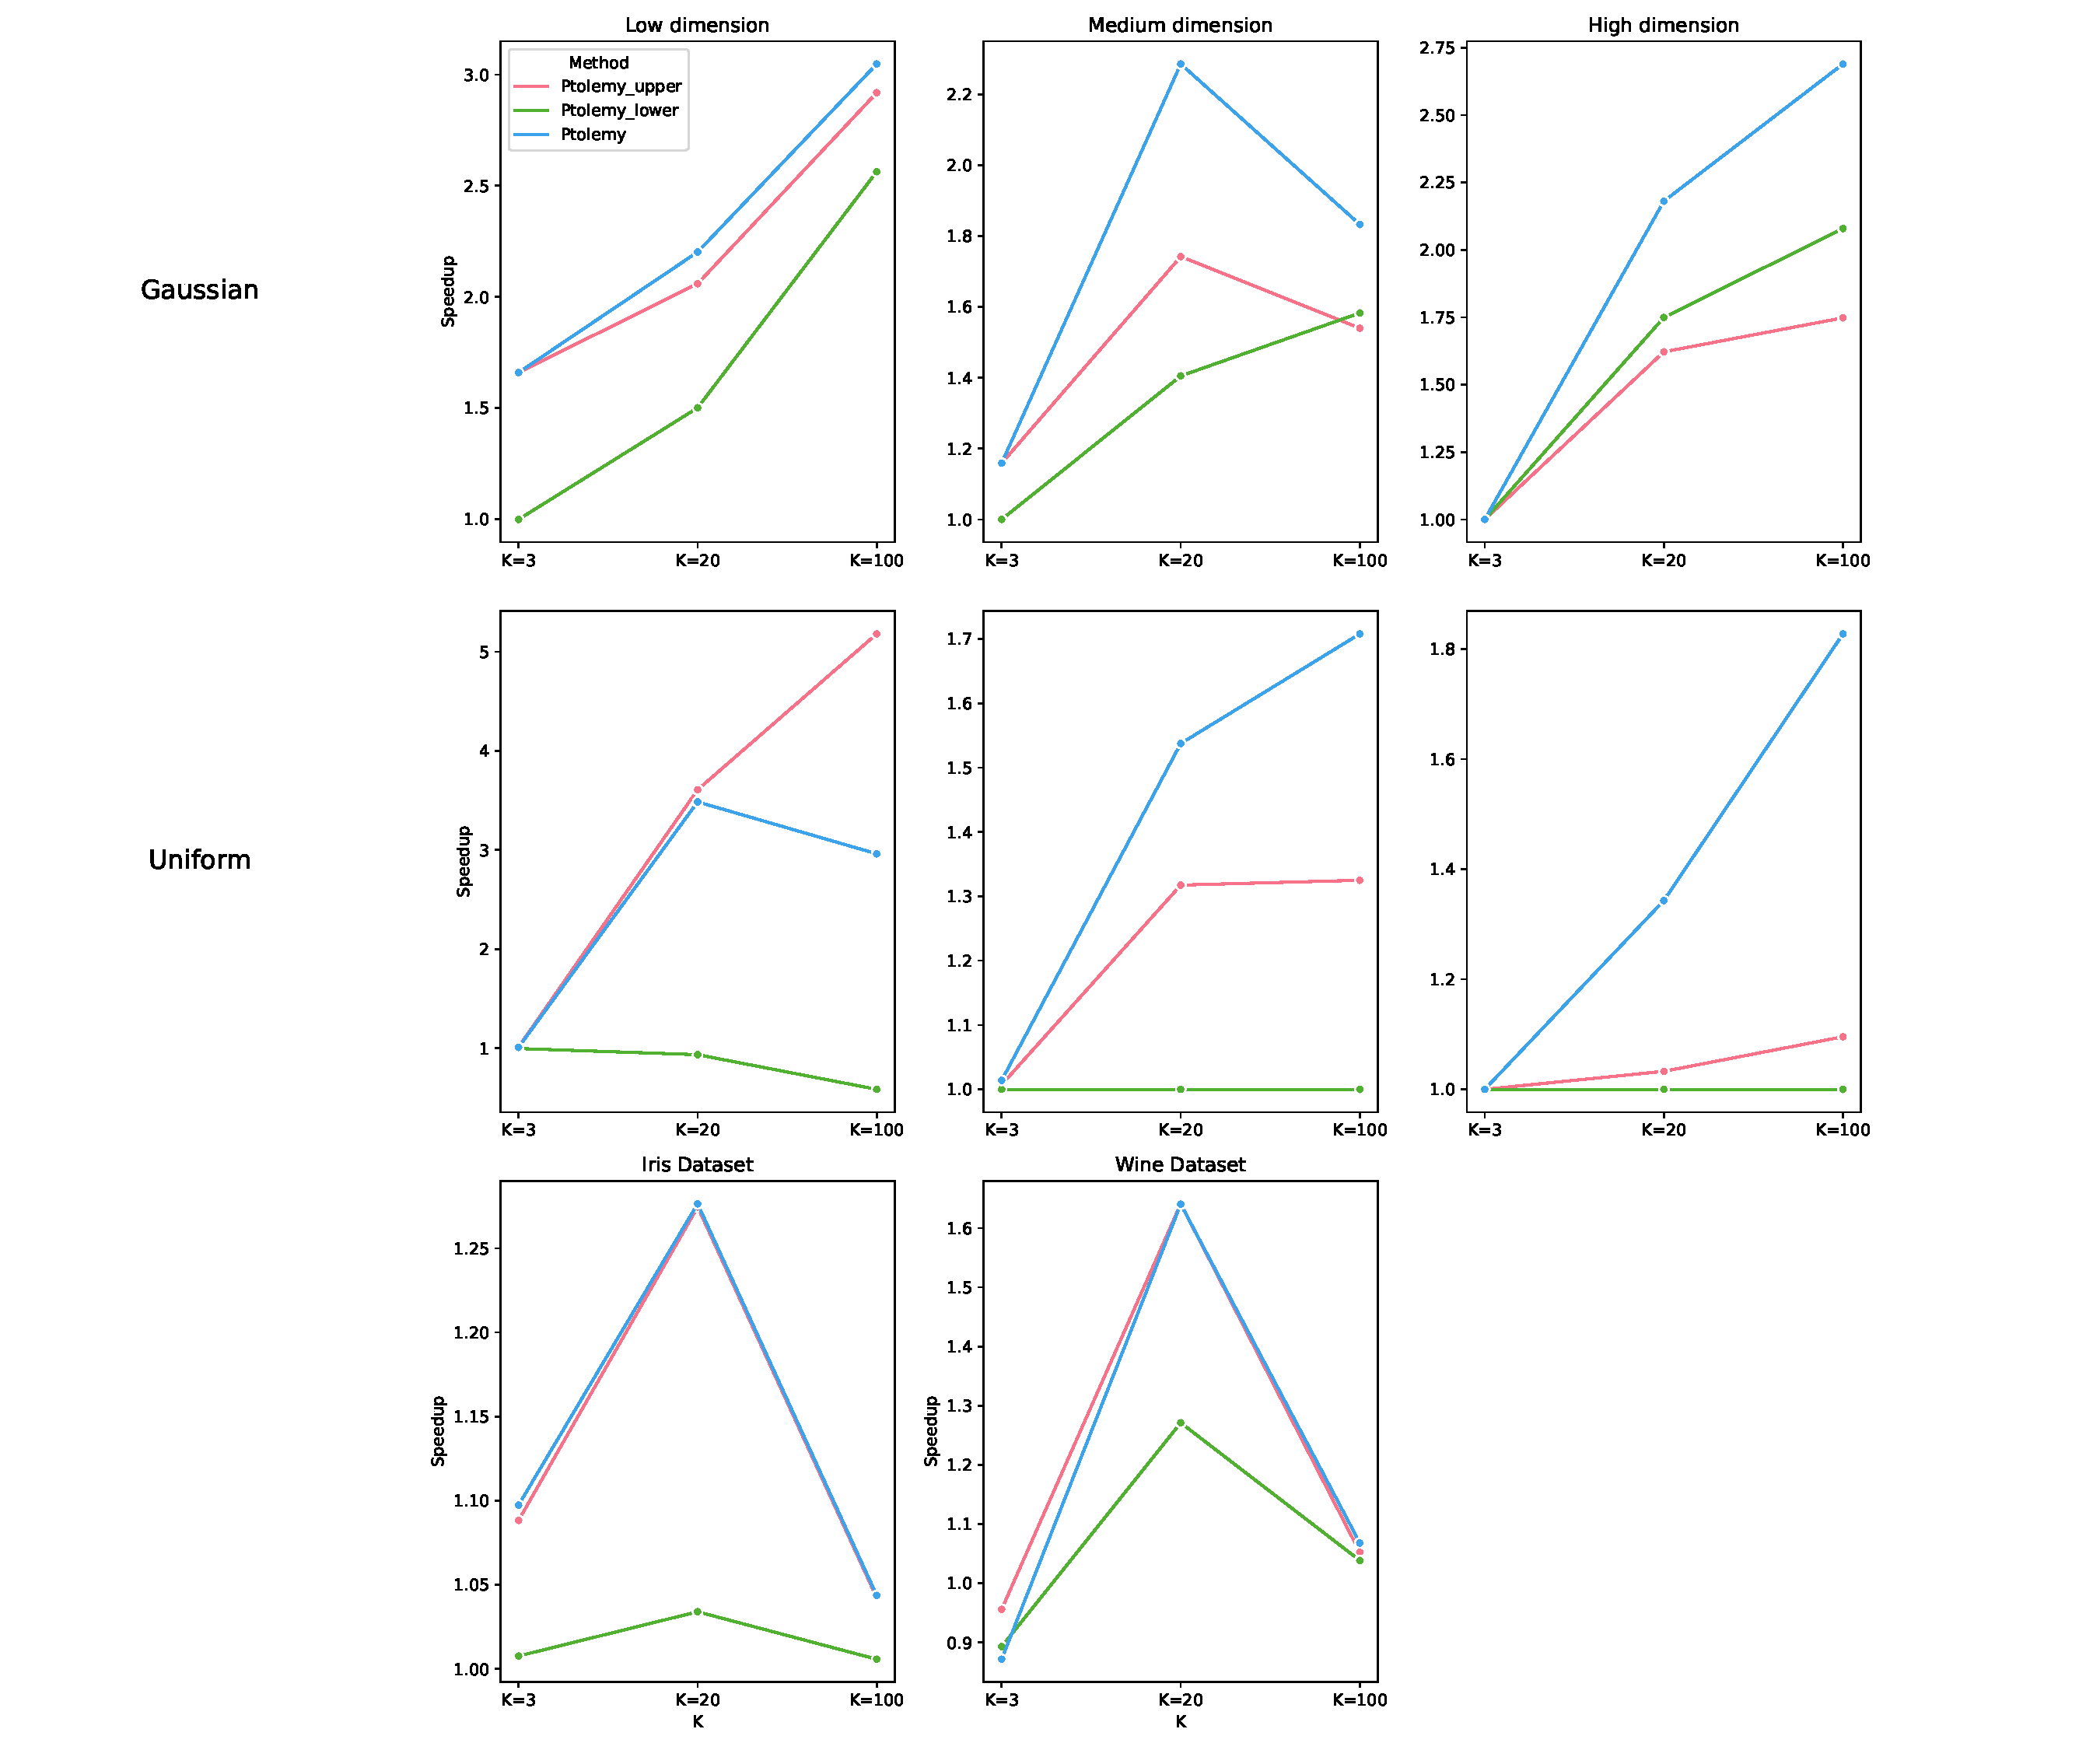
\includegraphics[width=\textwidth]{fig/combined_plot.pdf}
  \caption{}
  \label{fig:combined}
\end{figure}


\subsection{Analysis of the Results}

The experimental results, presented in the figures, provide critical insights into the performance of the k-Means algorithm variants. The primary focus of this analysis is on the full Ptolemaic algorithm and its comparison with Elkan’s algorithm. The results highlight several scenarios in which the full Ptolemaic algorithm achieves substantial improvements over Elkan’s approach, particularly in reducing the number of distance evaluations.

\textbf{Influence of the Number of Clusters}

The full Ptolemaic algorithm consistently demonstrates notable improvements over Elkan’s algorithm as the number of clusters ($k$) increases. For instance, in the Gaussian low-dimensional dataset, the Ptolemaic algorithm achieves speedups of over 2-fold for $k = 20$ and surpasses 3-fold for $k = 100$, illustrating its ability to significantly reduce distance calculations in more complex clustering tasks. Similar trends are observed in the Random low-dimensional dataset, where the full Ptolemaic algorithm achieves a speedup of more than 3-fold at $k = 20$ and $k = 100$. These results underscore the increasing efficiency of the Ptolemaic algorithm as the clustering complexity grows.

In contrast, for smaller cluster counts, such as $k = 3$, the performance advantage of the full Ptolemaic algorithm is less pronounced but still evident, with speedups of around 1.1 in both the Iris and Wine datasets. This suggests that while Ptolemy’s inequality offers significant improvements for larger $k$ values, it still provides moderate gains for smaller cluster sizes.

The Ptolemaic Upper Bound variant performs comparably to the full Ptolemaic algorithm, especially for larger $k$ values, delivering similar efficiency improvements. However, the Ptolemaic Lower Bound variant tends to underperform in some cases, particularly with smaller cluster counts or in higher-dimensional datasets, where its speedup is sometimes close to or even below that of Elkan’s algorithm.

\textbf{Influence of Dimensionality}

The full Ptolemaic algorithm also performs well across datasets with varying dimensionality. In the Gaussian low-dimensional dataset (10 dimensions), the full Ptolemaic algorithm achieves impressive speedups, particularly at higher cluster counts, with speedups over 3-fold at $k = 100$. As the dimensionality increases, the performance gains of the Ptolemaic algorithm persist, though they become slightly less pronounced. For example, in the Gaussian medium (100 dimensions) and Gaussian high (300 dimensions) datasets, the Ptolemaic algorithm continues to offer significant speedups, but the performance advantage over Elkan’s algorithm decreases slightly.

In higher-dimensional datasets, such as the Random high-dimensional dataset, the full Ptolemaic algorithm remains effective, consistently reducing the number of distance evaluations, particularly for larger $k$ values. However, the Ptolemaic Lower Bound variant often struggles in these higher-dimensional cases, further emphasizing the robustness of the full Ptolemaic approach.

\textbf{Summary of Results}

The full Ptolemaic algorithm demonstrates consistent and significant improvements over Elkan’s algorithm across a variety of datasets, particularly in scenarios with a high number of clusters and low to medium dimensionality. The Ptolemaic Upper Bound variant performs similarly in many cases, offering comparable efficiency gains, whereas the Ptolemaic Lower Bound variant sometimes struggles, particularly in datasets with higher dimensionality or smaller cluster counts. Overall, the full Ptolemaic algorithm proves to be a robust and efficient alternative to traditional k-Means implementations, especially as the complexity of the clustering task increases.


\section{Conclusions and Future Work} \label{sec: conclusions}

% This paper addresses efficient data clustering using the $k$-means algorithm.
% We extend Elkan's algorithm with novel distance approximations derived from Ptolemy's inequality.
% Preliminary evaluations show significant performance improvements over Elkan's method, particularly with large numbers of clusters at low-to-medium dimensionalities.
% The application of Ptolemy's inequality opens new avenues for future work, potentially enhancing other k-means algorithms that use triangle inequality for distance pruning. This approach could make clustering algorithms more practical across a broader range of applications.

This short paper has addressed the problem of efficient data clustering by means of the k-means algorithm.
We have shown how to extend the more efficient clustering algorithm proposed by Elkan with novel distance approximations derived from Ptolemy's inequality.
The results of our preliminary performance evaluation indicate that our proposal achieves significant improvements in performance compared to Elkan's algorithm. %Particularly noteworthy is the increased efficiency with a large number of clusters.

Moreover, the use of the Ptolemy's inequality opens up new avenues for future work.
Besides conducting more extensive experiments to verify our findings,
it would be valuable to explore adaptations of this technique for other k-means algorithms and optimizations.
In particular for algorithms which rely on the triangle inequality to prune distance calculations, Ptolemy's inequality can potentially be leveraged to achieve an enhancement in performance, making these clustering algorithms more practical for a broader range of applications.

% \todo{Moreover, the use of Ptolemy’s inequality opens new avenues for future work. Exploring adaptations of this technique for other K-Means algorithms and optimizations could be highly valuable. In particular, algorithms that rely on the triangle inequality to prune distance calculations might leverage Ptolemy’s inequality to enhance performance, making these clustering algorithms more practical for a broader range of applications.}

\bibliography{references,bibliography_thesis,bibliography_iiwas}
\end{document}
